\section*{Kapitel 4 - Diskrete Einflußgrößen}

\begin{multicols*}{3}

\tikzstyle{mybox} = [draw=black, fill=white, very thick,
    rectangle, rounded corners, inner sep=10pt, inner ysep=10pt]
\tikzstyle{fancytitle} =[fill=black, text=white, font=\bfseries]



%------------ Kodierung ---------------
\begin{tikzpicture}
    \node [mybox] (box){%
        \begin{minipage}{0.3\textwidth}
        Sei $C$ eine nominale Variable mit $K$ Ausprägungen.
        \vspace{0.5cm}

        \tc{\textbf{Dummy/Referenz-Kodierung:}}\\
         Wir definieren $K$ neue Variablen $Z_1, \dots, Z_K$ als
         $$Z_k(C) = \begin{cases} 1, & \text{falls } C = k \\ 0, & \text{sonst} \end{cases}$$
         $Z_1, \dots, Z_K$ sind abhängig, da $Z_K = 1 - \sum_{k=1}^{K-1} Z_k$
        \vspace{0.5cm}

        \tc{\textbf{Effekt-Kodierung:}}
        Wir definieren $K-1$ neue Variablen $Z_1^e, \dots, Z_{K-1}^e$ als
        $$Z_k^e(C) = \begin{cases} 1, & \text{falls } C = k \\ -1, & \text{falls } C = K \\ 0, & \text{sonst} \end{cases}$$
        Note: $Z_k(\bC) = \begin{pmatrix}
            Z_k(C_1) \\ \vdots \\ Z_k(C_n) \end{pmatrix}$ und $Z_k^e(\bC) = \begin{pmatrix}
                Z_k^e(C_1) \\ \vdots \\ Z_k^e(C_n) \end{pmatrix}$
    \end{minipage}
    };
%------------ Kodierung Header ---------------------
\node[fill = black, text=white, font=\bfseries, right=10pt] at (box.north west) 
{Kodierung};
\end{tikzpicture}

%------------ Setup einfache Varianzanalyse ---------------
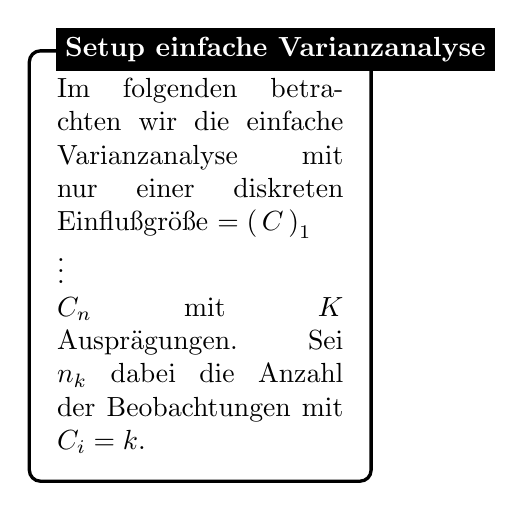
\begin{tikzpicture}
    \node [mybox] (box){%
        \begin{minipage}{0.3\textwidth}
        Im folgenden betrachten wir die einfache Varianzanalyse mit nur einer diskreten Einflußgröße 
        $\bC = \begin{pmatrix} C_1 \\ \vdots \\ C_n \end{pmatrix}$ mit $K$ Ausprägungen.
        Sei $n_k$ dabei die Anzahl der Beobachtungen mit $C_i = k$.
        \end{minipage}
    };
%------------ Setup einfache Varianzanalyse Header ---------------------
\node[fill = black, text=white, font=\bfseries, right=10pt] at (box.north west) 
{Setup einfache Varianzanalyse};
\end{tikzpicture}


%------------ Mittelwertsmodell ---------------
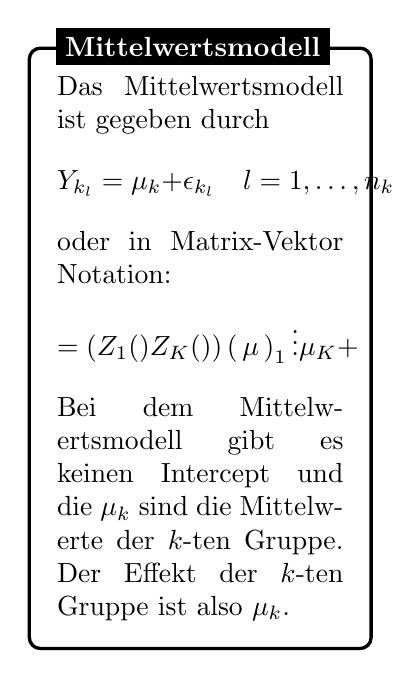
\begin{tikzpicture}
    \node [mybox] (box){%
        \begin{minipage}{0.3\textwidth}
        Das \tc{Mittelwertsmodell} ist gegeben durch
        $$Y_{k_l} = \mu_k + \epsilon_{k_l} \quad l = 1,\dots, n_k \quad k = 1,\dots,K$$
        oder in Matrix-Vektor Notation: 
        $$\bY = (Z_1(\bC) \dotsm Z_K(\bC)) \begin{pmatrix}
            \mu_1 \\ \vdots \\ \mu_K
        \end{pmatrix} + \bepsilon$$
        Bei dem Mittelwertsmodell gibt es keinen Intercept und die $\mu_k$ sind die Mittelwerte der $k$-ten Gruppe.
        Der Effekt der $k$-ten Gruppe ist also $\mu_k$.
        \end{minipage}
    };
%------------ Mittelwertsmodell Header ---------------------
\node[fill = black, text=white, font=\bfseries, right=10pt] at (box.north west) 
{Mittelwertsmodell};
\end{tikzpicture}

%------------ Mittelwertsmodell Beispiel ---------------
\begin{tikzpicture}
    \node [mybox] (box){%
        \begin{minipage}{0.3\textwidth}
        Für $K = 3$ Ausprägungen und $n_k = 2$ für alle $k=1,2,3$ erhalten wir als Mittelwertsmodell:
        $$\bY = \begin{pmatrix} Y_{1_1} \\ Y_{1_2} \\ Y_{2_1} \\ Y_{2_2} \\ Y_{3_1} \\ Y_{3_2}
         \end{pmatrix} = \begin{pmatrix}
            1 & 0 & 0 \\ 1 & 0 & 0 \\ 0 & 1 & 0 \\ 0 & 1 & 0 \\ 0 & 0 & 1 \\ 0 & 0 & 1 \end{pmatrix} \begin{pmatrix}
                \mu_1 \\ \mu_2 \\ \mu_3 \end{pmatrix} + \begin{pmatrix}
                    \eps_{1_1} \\ \eps_{1_2} \\ \eps_{2_1} \\ \eps_{2_2} \\ \eps_{3_1} \\ \eps_{3_2}
        \end{pmatrix}$$
        \end{minipage}
    };
%------------ Mittelwertsmodell Beispiel Header ---------------------
\node[fill = blue, text=white, font=\bfseries, right=10pt] at (box.north west) 
{Mittelwertsmodell Beispiel};
\end{tikzpicture}


%------------ Modell mit Effekt-Kodierung ---------------
\begin{tikzpicture}
    \node [mybox] (box){%
        \begin{minipage}{0.3\textwidth}
        Das \tc{Modell mit Effekt-Kodierung} ist gegeben durch
        $$Y_{k_l} = \mu + \tau_k + \epsilon_{k_l}; \quad \tau_K = -\sum_{k = 1}^{K-1} \tau_k$$ 
        für $\quad l = 1,\dots, n_k \quad k = 1,\dots,K$
        oder in Matrix-Vektor Notation: 
        $$\bY = (\be \hspace{2mm} Z_1^e(\bC) \dotsm Z_{K-1}^e(\bC)) \begin{pmatrix}
            \mu \\ \tau_1 \\ \vdots \\ \tau_{K-1}
        \end{pmatrix} + \bepsilon$$
        Bei dem Modell mit Effekt-Kodierung gibt es einen Intercept $\mu$ und die $\tau_k$ sind die Abweichungen der $k$-ten Gruppe vom Gesamtmittelwert bzw. vom Intercept $\mu$.
        Der Effekt der $k$-ten Gruppe ist also $\mu + \tau_k$.
        \end{minipage}
    };
%------------ Modell mit Effekt-Kodierung Header ---------------------
\node[fill = black, text=white, font=\bfseries, right=10pt] at (box.north west) 
{Modell mit Effekt-Kodierung};
\end{tikzpicture}

%------------ Modell mit Effekt-Kodierung Beispiel ---------------
\begin{tikzpicture}
    \node [mybox] (box){%
        \begin{minipage}{0.3\textwidth}
        Für $K = 3$ Ausprägungen und $n_k = 2$ für alle $k=1,2,3$ erhalten wir als Modell mit Effekt-Kodierung:
        $$\bY = \begin{pmatrix} Y_{1_1} \\ Y_{1_2} \\ Y_{2_1} \\ Y_{2_2} \\ Y_{3_1} \\ Y_{3_2}
         \end{pmatrix} = \begin{pmatrix}
            1 & 1 & 0 \\ 1 & 1 & 0 \\ 1 & 0 & 1 \\ 1 & 0 & 1 \\ 1 & -1 & -1 \\ 1 & -1 & -1 \end{pmatrix} \begin{pmatrix}
                \mu \\ \tau_1 \\ \tau_2  \end{pmatrix}
         + \begin{pmatrix}
            \eps_{1_1} \\ \eps_{1_2} \\ \eps_{2_1} \\ \eps_{2_2} \\ \eps_{3_1} \\ \eps_{3_2} \end{pmatrix}$$
                \end{minipage}
    };
%------------ Modell mit Effekt-Kodierung Beispiel Header ---------------------
\node[fill = blue, text=white, font=\bfseries, right=10pt] at (box.north west) 
{Modell mit Effekt-Kodierung Beispiel};
\end{tikzpicture}

%------------ Modell mit Referenz-Kodierung ---------------
\begin{tikzpicture}
    \node [mybox] (box){%
        \begin{minipage}{0.3\textwidth}
        Das \tc{Modell mit Referenz-Kodierung} ist gegeben durch
        $$Y_{k_l} = \mu_K + \tau_k + \epsilon_{k_l}; \quad \tau_K = 0$$ 
        für $\quad l = 1,\dots, n_k \quad k = 1,\dots,K$
        oder in Matrix-Vektor Notation:
        $$\bY = (\be \hspace{2mm} Z_1(\bC) \dotsm Z_{K-1}(\bC)) \begin{pmatrix}
            \mu_K \\ \tau_1 \\ \vdots \\ \tau_{K-1}
        \end{pmatrix} + \bepsilon$$
        Beim Modell mit Referenz-Kodierung gibt es einen Intercept $\mu_K$ der den Mittelwert der $K$-ten Gruppe angibt und die $\tau_k$ sind die Abweichungen der $k$-ten Gruppe vom Mittelwert der $K$-ten Referenz-Gruppe.
        Der Effekt der $k$-ten Gruppe ist also $\mu_K + \tau_k$ für $k = 1,\dots,K-1$ und $\mu_K$ für $k = K$.
        \end{minipage}
    };
%------------ Modell mit Referenz-Kodierung Header ---------------------
\node[fill = black, text=white, font=\bfseries, right=10pt] at (box.north west) 
{Modell mit Referenz-Kodierung};
\end{tikzpicture}

%------------ Modell mit Referenz-Kodierung Beispiel ---------------
\begin{tikzpicture}
    \node [mybox] (box){%
        \begin{minipage}{0.3\textwidth}
        Für $K = 3$ Ausprägungen und $n_k = 2$ für alle $k=1,2,3$ erhalten wir als Modell mit Referenz-Kodierung:
        $$\bY = \begin{pmatrix} Y_{1_1} \\ Y_{1_2} \\ Y_{2_1} \\ Y_{2_2} \\ Y_{3_1} \\ Y_{3_2}
         \end{pmatrix} = \begin{pmatrix}
            1 & 1 & 0 \\ 1 & 1 & 0 \\ 1 & 0 & 1 \\ 1 & 0 & 1 \\ 1 & 0 & 0 \\ 1 & 0 & 0 \end{pmatrix} \begin{pmatrix}
                \mu_3 \\ \tau_1 \\ \tau_2  \end{pmatrix}
         + \begin{pmatrix}
            \eps_{1_1} \\ \eps_{1_2} \\ \eps_{2_1} \\ \eps_{2_2} \\ \eps_{3_1} \\ \eps_{3_2} \end{pmatrix}$$
                \end{minipage}
    };
%------------ Modell mit Referenz-Kodierung Beispiel Header ---------------------
\node[fill = blue, text=white, font=\bfseries, right=10pt] at (box.north west) 
{Modell mit Referenz-Kodierung Beispiel};
\end{tikzpicture}

%------------ Bemerkungen-Kodierung ---------------
\begin{tikzpicture}
    \node [mybox] (box){%
        \begin{minipage}{0.3\textwidth}
        Alle Modellvarianten führen zur gleichen Modellanpassung ($R^2$).
        Die Parameter haben aber unterschiedliche Interpretationen. Parameter und deren Schätzer sind aber ineinander umrechenbar.

        Wir können folgende Nullhypothese für den Effekt von $C$ testen:
        \begin{align*}
            & \text{Mittelwertsmodell \quad} & H_0: & \mu_1 = \dots = \mu_K \\
            & \text{Effekt-Kodierung \quad} & H_0: & \tau_1 = \dots = \tau_{K-1} = 0\\
            & \text{Referenz-Kodierung \quad} & H_0: & \tau_1 = \dots = \tau_{K-1} = 0
        \end{align*}
        \end{minipage}
    };
%------------ Bemerkungen-Kodierung Header ---------------------
\node[fill = purple, text=white, font=\bfseries, right=10pt] at (box.north west) 
{Bemerkungen-Kodierung};
\end{tikzpicture}

\newpage

%------------ Setup einfache Varianzanalyse ---------------
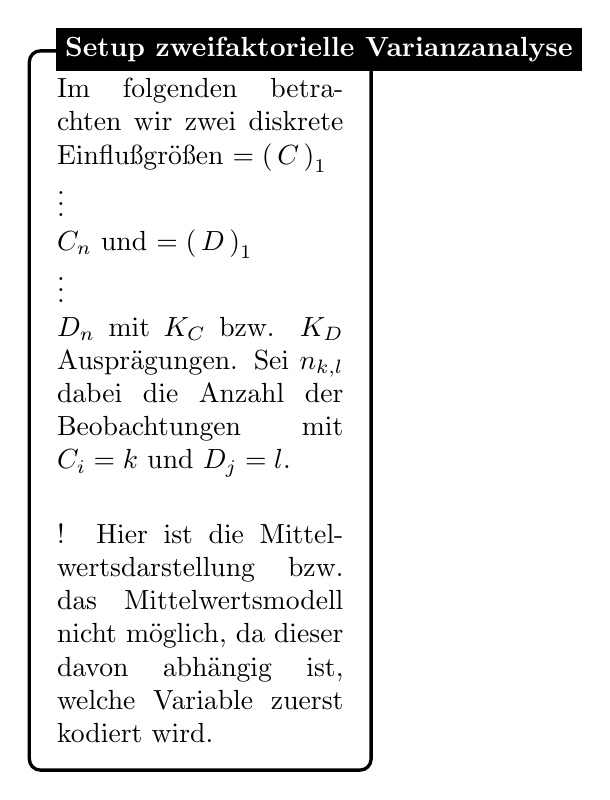
\begin{tikzpicture}
    \node [mybox] (box){%
        \begin{minipage}{0.3\textwidth}
        Im folgenden betrachten wir zwei diskrete Einflußgrößen $\bC = \begin{pmatrix} C_1 \\ \vdots \\ C_n \end{pmatrix}$ und 
        $\bD = \begin{pmatrix} D_1 \\ \vdots \\ D_n \end{pmatrix}$ mit $K_C$ bzw. $K_D$ Ausprägungen.
        Sei $n_{k,l}$ dabei die Anzahl der Beobachtungen mit $C_i = k$ und $D_j = l$.\\
        \vspace{1mm}

        \tc{!} Hier ist die Mittelwertsdarstellung bzw. das Mittelwertsmodell nicht möglich, da dieser davon abhängig ist, welche Variable zuerst kodiert wird.
        \end{minipage}
    };
%------------ Setup einfache Varianzanalyse Header ---------------------
\node[fill = black, text=white, font=\bfseries, right=10pt] at (box.north west) 
{Setup zweifaktorielle Varianzanalyse};
\end{tikzpicture}

%------------ Modell mit Effekt-Kodierung (mehrfaktoriell) ---------------
\begin{tikzpicture}
    \node [mybox] (box){%
        \begin{minipage}{0.3\textwidth}
        Das \tc{Modell mit Effekt-Kodierung} ist gegeben durch
        \tiny{
            $$\bY = (\be \hspace{2mm} Z_1^e(\bC) \dotsm Z_{K_C-1}^e(\bC) \hspace{2mm} Z_1^e(\bD) \dotsm Z_{K_D-1}^e(\bD)) \begin{pmatrix}
            \mu \\ \tau_1 \\ \vdots \\ \tau_{K_C-1} \\ \gamma_1 \\ \vdots \\ \gamma_{K_D-1} \end{pmatrix} + \bepsilon$$\\
        }
        \normalsize{
        mit $\tau_{K_C} = -\sum_{k = 1}^{K_C-1} \tau_k$ und $\gamma_{K_D} = -\sum_{k = 1}^{K_D-1} \gamma_k$.
        }
        \vspace{2mm}

        Bei dem Modell mit Effekt-Kodierung gibt es einen Intercept $\mu$ und die $\tau_k$ und $\gamma_l$
        sind die Abweichungen der Gruppe mit $C = k$ bzw. $D = l$ vom Gesamtmittelwert bzw. vom Intercept $\mu$.
        \end{minipage}
    };
%------------ Modell mit Effekt-Kodierung (mehrfaktoriell) Header ---------------------
\node[fill = black, text=white, font=\bfseries, right=10pt] at (box.north west) 
{Modell mit Effekt-Kodierung (mehrfaktoriell)};
\end{tikzpicture}

%------------ Modell mit Referenz-Kodierung (mehrfaktoriell) ---------------
\begin{tikzpicture}
    \node [mybox] (box){%
        \begin{minipage}{0.3\textwidth}
        Das \tc{Modell mit Referenz-Kodierung} ist gegeben durch
        \tiny{
            $$\bY = (\be \hspace{2mm} Z_1(\bC) \dotsm Z_{K_C-1}(\bC) \hspace{2mm} Z_1(\bD) \dotsm Z_{K_D-1}(\bD)) \begin{pmatrix}
            \mu \\ \tau_1 \\ \vdots \\ \tau_{K_C-1} \\ \gamma_1 \\ \vdots \\ \gamma_{K_D-1} \end{pmatrix} + \bepsilon$$\\
        }
        \normalsize{
        mit $\tau_{K_C} = 0$ und $\gamma_{K_D} = 0$.
        }
        \vspace{2mm}

        Bei dem Modell mit Referenz-Kodierung gibt es einen Intercept $\mu$ der den Mittelwert der Gruppe mit $C = K_C$ und $D = K_D$ angibt
        und die $\tau_k$ und $\gamma_l$ sind die Abweichungen der Gruppe mit $C = k$ bzw. $D = l$ vom Mittelwert der Gruppe mit $C = K_C$ und $D = K_D$.
        \end{minipage}
    };
%------------ Modell mit Referenz-Kodierung (mehrfaktoriell) Header ---------------------
\node[fill = black, text=white, font=\bfseries, right=10pt] at (box.north west) 
{Modell mit Referenz-Kodierung (mehrfakt.)};
\end{tikzpicture}

%------------ Kodierung Vergleich (mehrfaktoriell) Beispiel---------------
\begin{tikzpicture}
    \node [mybox] (box){%
        \begin{minipage}{0.3\textwidth}
        Sei $K_C = 2$ und $K_D = 3$ mit $n_{k,l} = 2$ für alle $k=1,2,3$ und $l=1,2$.\\
        Dann erhalten wir als Designmatrix für das Modell mit \\
        \vspace{2mm}

        \textbf{Effekt-Kodierung}:
        $$\bX = (\be \hspace{1mm} Z_1^e(\bC) \hspace{1 mm} Z_1^e(\bD) \hspace{1mm} Z_2^e(\bD)) = \begin{pmatrix}
            1 & 1 & 1 & 0 \\ 1 & 1 & 1 & 0 \\ 1 & 1 & 0 & 1 \\ 1 & 1 & 0 & 1 \\ 1 & 1 & -1 & -1 \\ 1 & 1 & -1 & -1 \\
            1 & -1 & 1 & 0 \\ 1 & -1 & 1 & 0 \\ 1 & -1 & 0 & 1 \\ 1 & -1 & 0 & 1 \\ 1 & -1 & -1 & -1 \\ 1 & -1 & -1 & -1 
        \end{pmatrix}$$

        \vspace{2mm}
        \textbf{Referenz-Kodierung}:
        $$\bX = (\be \hspace{1mm} Z_1(\bC) \hspace{1 mm} Z_1(\bD) \hspace{1mm} Z_2(\bD)) = \begin{pmatrix}
            1 & 1 & 1 & 0 \\ 1 & 1 & 1 & 0 \\ 1 & 1 & 0 & 1 \\ 1 & 1 & 0 & 1 \\ 1 & 1 & 0 & 0 \\ 1 & 1 & 0 & 0 \\
            1 & 0 & 1 & 0 \\ 1 & 0 & 1 & 0 \\ 1 & 0 & 0 & 1 \\ 1 & 0 & 0 & 1 \\ 1 & 0 & 0 & 0 \\ 1 & 0 & 0 & 0
        \end{pmatrix}$$
        \end{minipage}
    };
%------------ Modell mit Kodierung Vergleich (mehrfaktoriell) Beispiel Header ---------------------
\node[fill = blue, text=white, font=\bfseries, right=10pt] at (box.north west) 
{Kodierung Vergleich (mehrfaktoriell) Beispiel};
\end{tikzpicture}

%------------ Visualisierung Beispiel---------------
\begin{tikzpicture}
    \node [mybox] (box){%
        \begin{minipage}{0.3\textwidth}
        Wir können die Effekte visualisieren, indem wir die Mittelwerte der Gruppen betrachten:
        \begin{center}
            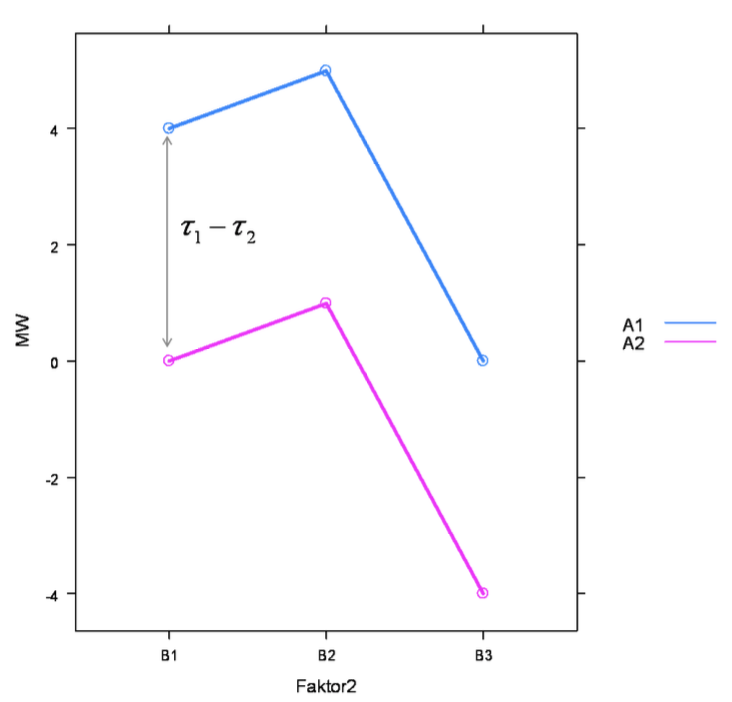
\includegraphics[width=0.8\linewidth]{fig/Effekt_Plot.png} 
        \end{center}

        Note: "Faktor 2" ist hier $D$ und "A1" und "A2" sind hier $C = 1$ und $C=2$.
        Auf der y-Achse ist der Mittelwert der Gruppe dargestellt.\\
        \vspace{2mm}

        In beiden Fällen werden folgende Gleichungen erfüllt:
        \begin{align*}
        %&\mu + \tau_1 + \gamma_1 = 4 & \mu + \tau_2 + \gamma_1 = &0\\
        %&\mu + \tau_1 + \gamma_2 = 5 & \mu + \tau_2 + \gamma_2 = &1\\
        %&\mu + \tau_1 + \gamma_3 = 0 & \mu + \tau_2 + \gamma_3 = &-4
        % Same code as above but with \wh{} before every parameter
        &\wh{\mu} + \wh{\tau_1} + \wh{\gamma_1} = 4 & \wh{\mu} + \wh{\tau_2} + \wh{\gamma_1} = &0\\
        &\wh{\mu} + \wh{\tau_1} + \wh{\gamma_2} = 5 & \wh{\mu} + \wh{\tau_2} + \wh{\gamma_2} = &1\\
        &\wh{\mu} + \wh{\tau_1} + \wh{\gamma_3} = 0 & \wh{\mu} + \wh{\tau_2} + \wh{\gamma_3} = &-4
        \end{align*}

        \textbf{Effekt-Kodierung:}
        \begin{align*}
        \wh{\mu} &= 1 & \wh{\gamma_1} &= 1\\
        \wh{\tau_1} &= 2 & \wh{\gamma_2} &= 2\\
        \wh{\tau_2} &= -2 & \wh{\gamma_3} &= -3
        \end{align*}
        
        \tc{!} Der Verlauf für $C = 1$ und $C = K_C = 2$ ist parallel mit Abstand $\wh{\tau_1} - \wh{\tau_2}$.
        \vspace{2mm}

        \textbf{Referenz-Kodierung:}
        \begin{align*}
        & \wh{\mu} = -4  & \wh{\gamma_1} &= 4\\
        & \wh{\tau_1} = 4 & \wh{\gamma_2} &= 5\\
        & \wh{\tau_2} = 0 & \wh{\gamma_3} &= 0
        \end{align*}

        \tc{!} Der Verlauf für $C = 1$ und $C = K_C = 2$ ist parallel mit Abstand $\wh{\tau_1}$.
        Man beachte auch, dass sich die Schätzer direkt in dem Plot ablesen lassen.
        \end{minipage}
    };
%------------ Visualisierung Beispiel Header ---------------------
\node[fill = blue, text=white, font=\bfseries, right=10pt] at (box.north west) 
{Visualisierung Beispiel};
\end{tikzpicture}

%------------ Interaktion ---------------
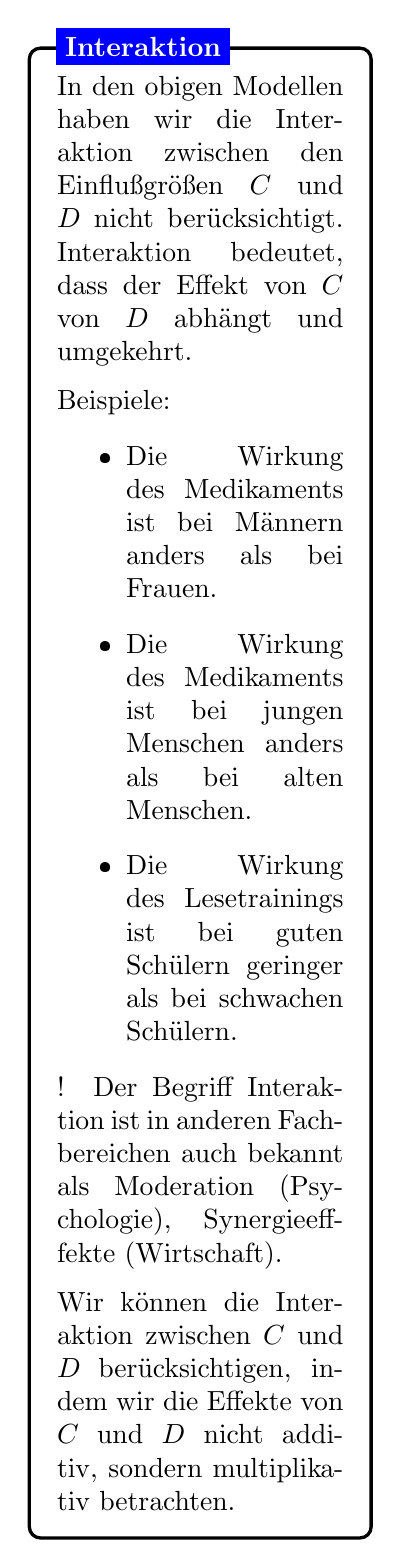
\begin{tikzpicture}
    \node [mybox] (box){%
        \begin{minipage}{0.3\textwidth}
        In den obigen Modellen haben wir die Interaktion zwischen den Einflußgrößen $C$ und $D$ nicht berücksichtigt.
        Interaktion bedeutet, dass der Effekt von $C$ von $D$ abhängt und umgekehrt.
        \vspace{2mm}

        Beispiele:
        \begin{itemize}
            \item Die Wirkung des Medikaments ist bei Männern anders als bei Frauen.
            \item Die Wirkung des Medikaments ist bei jungen Menschen anders als bei alten Menschen.
            \item Die Wirkung des Lesetrainings ist bei guten Schülern geringer als bei schwachen Schülern.
        \end{itemize}

        \tc{!} Der Begriff Interaktion ist in anderen Fachbereichen auch bekannt als Moderation (Psychologie), Synergieefffekte (Wirtschaft).
        \vspace{2mm}

        Wir können die Interaktion zwischen $C$ und $D$ berücksichtigen, indem wir die Effekte von $C$ und $D$ nicht additiv, sondern multiplikativ betrachten.
        \end{minipage}
    };
%------------ Interaktion Header ---------------------
\node[fill = blue, text=white, font=\bfseries, right=10pt] at (box.north west) 
{Interaktion};
\end{tikzpicture}

%------------ Interaktionsmodell (Effekt-Kodierung) ---------------
\begin{tikzpicture}
    \node [mybox] (box){%
        \begin{minipage}{0.3\textwidth}
        In dem \tc{Modell mit Effekt-Kodierung und Interaktion} ist die Designmatrix gegeben durch die Spalten der Designmatrix aus dem Modell ohne Interaktion $\bX^e$ und zusätzlich die Spalten der Interaktionsterme:
        \tiny{
            $$\bZ^e = (Z_1^e(\bC)Z_1^e(\bD) \dotsm Z_1^e(\bC)Z_{K_D-1}^e(\bD) \dotsm Z_{K_C-1}^e(\bC)Z_{K_D-1}^e(\bD))$$
        }\\
        \normalsize{
        Die Designmatrix ist also gegeben durch $\begin{pmatrix}
            \bX^e & \bZ^e
        \end{pmatrix}$
        }
        \vspace{2mm}
        
        Die Parameter sind gegeben durch
        $\mu \quad \tau_k \quad \gamma_l \quad (\tau \gamma)_{k,l}$\\ mit 
        $k = 1,\dots,K_C-1 \quad l = 1,\dots,K_D-1$.
        \vspace{2mm}

        Die Modellgleichung ist gegeben durch
        $$Y_{k,l} = \mu + \tau_k + \gamma_l + (\tau \gamma)_{k,l} + \epsilon_{k,l}$$
        mit den Nebenbedingungen
        $$\sum_{k=1}^{K_C-1} \tau_k = 0 \quad \text{und} \quad \sum_{l=1}^{K_D-1} \gamma_l = 0$$
        sowie 
        $$\forall l: \sum_{k=1}^{K_C} (\tau \gamma)_{k,l} = 0 \quad \text{und} \quad \forall k: \sum_{l=1}^{K_D} (\tau \gamma)_{k,l} = 0$$
        
        \end{minipage}
    };
%------------ Interaktionsmodell (Effekt-Kodierung) Header ---------------------
\node[fill = black, text=white, font=\bfseries, right=10pt] at (box.north west) 
{Interaktionsmodell (Effekt-Kodierung)};
\end{tikzpicture}

%------------ Interaktionsmodell Interpretation ---------------
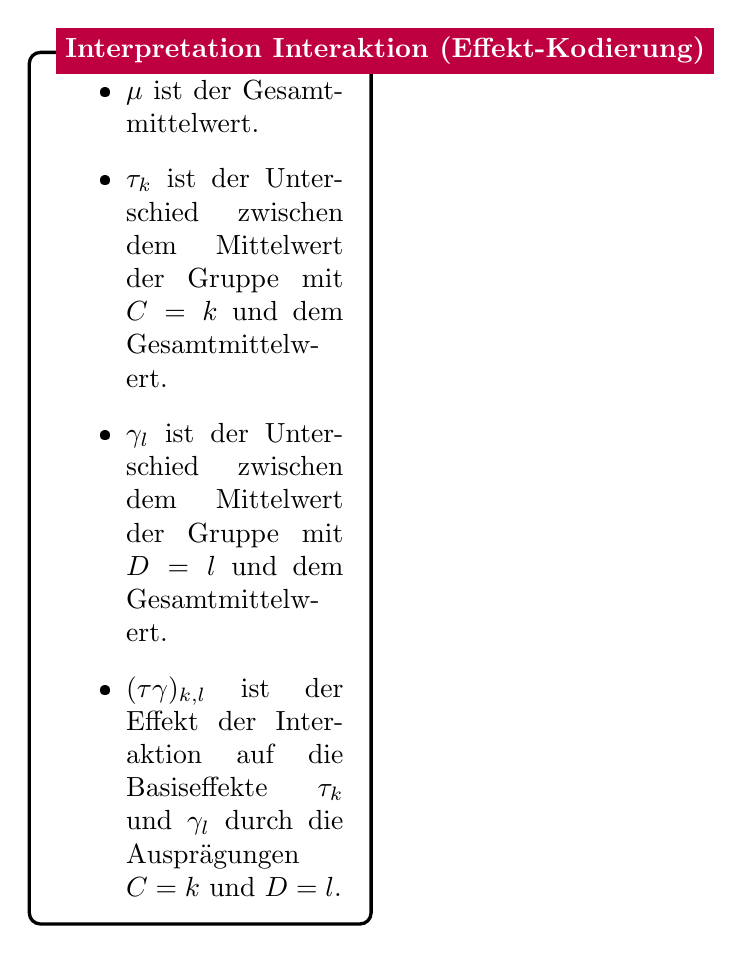
\begin{tikzpicture}
    \node [mybox] (box){%
        \begin{minipage}{0.3\textwidth}
        \begin{itemize}
            \item $\mu$ ist der Gesamtmittelwert.
            \item $\tau_k$ ist der Unterschied zwischen dem Mittelwert der Gruppe mit $C = k$ und dem Gesamtmittelwert.
            \item $\gamma_l$ ist der Unterschied zwischen dem Mittelwert der Gruppe mit $D = l$ und dem Gesamtmittelwert.
            \item $(\tau \gamma)_{k,l}$ ist der Effekt der Interaktion auf die Basiseffekte $\tau_k$ und $\gamma_l$ durch die Ausprägungen $C = k$ und $D = l$. 
        \end{itemize}
        \end{minipage}
    };
%------------ Interaktionsmodell Interpretation Header ---------------------
\node[fill = purple, text=white, font=\bfseries, right=10pt] at (box.north west) 
{Interpretation Interaktion (Effekt-Kodierung) };
\end{tikzpicture}

%------------ Interaktionsmodell (Referenz-Kodierung)---------------
\begin{tikzpicture}
    \node [mybox] (box){%
        \begin{minipage}{0.3\textwidth}
        In dem \tc{Modell mit Referenz-Kodierung und Interaktion} ist die Designmatrix gegeben durch die Spalten der Designmatrix aus dem Modell ohne Interaktion $\bX$ und zusätzlich die Spalten der Interaktionsterme:
        \tiny{
            $$\bZ = (Z_1(\bC)Z_1(\bD) \dotsm Z_1(\bC)Z_{K_D-1}(\bD) \dotsm Z_{K_C-1}(\bC)Z_{K_D-1}(\bD))$$
        }
        \normalsize{
        Die Designmatrix ist also gegeben durch $\begin{pmatrix}
            \bX & \bZ
        \end{pmatrix}$.
        }
        \vspace{2mm}
        
        Die Parameter sind gegeben durch
        $\mu \quad \tau_k \quad \gamma_l \quad (\tau \gamma)_{k,l}$\\ mit 
        $k = 1,\dots,K_C-1 \quad l = 1,\dots,K_D-1$.
        \vspace{2mm}

        Die Modellgleichung ist gegeben durch
        $$Y_{k,l} = \mu + \tau_k + \gamma_l + (\tau \gamma)_{k,l} + \epsilon_{k,l}$$
        mit den Nebenbedingungen
        $$\tau_{K_C} = 0 \quad \text{und} \quad \gamma_{K_D} = 0$$
        sowie
        $$\forall l: (\tau \gamma)_{K_C,l} = 0 \quad \text{und} \quad \forall k: (\tau \gamma)_{k,K_D} = 0$$
        
        \end{minipage}
    };
%------------ Interaktionsmodell (Referenz-Kodierung) Header ---------------------
\node[fill = black, text=white, font=\bfseries, right=10pt] at (box.north west) 
{Interaktionsmodell (Referenz-Kodierung)};
\end{tikzpicture}

%------------ Interaktionsmodell Interpretation ---------------
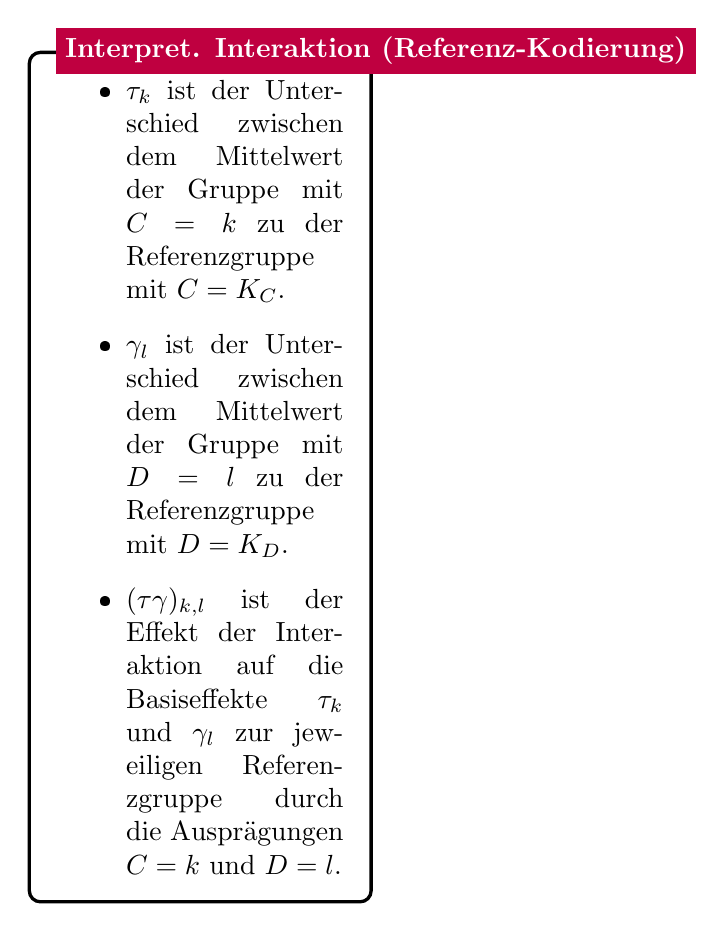
\begin{tikzpicture}
    \node [mybox] (box){%
        \begin{minipage}{0.3\textwidth}
        \begin{itemize}
            \item $\tau_k$ ist der Unterschied zwischen dem Mittelwert der Gruppe mit $C = k$ zu der Referenzgruppe mit $C = K_C$.
            \item $\gamma_l$ ist der Unterschied zwischen dem Mittelwert der Gruppe mit $D = l$ zu der Referenzgruppe mit $D = K_D$.
            \item $(\tau \gamma)_{k,l}$ ist der Effekt der Interaktion auf die Basiseffekte $\tau_k$ und $\gamma_l$ zur jeweiligen Referenzgruppe durch die Ausprägungen $C = k$ und $D = l$.
        \end{itemize}
        \end{minipage}
    };
%------------ Interaktionsmodell Interpretation Header ---------------------
\node[fill = purple, text=white, font=\bfseries, right=10pt] at (box.north west) 
{Interpret. Interaktion (Referenz-Kodierung) };
\end{tikzpicture}

%------------ Visualisierung Beispiel---------------
\begin{tikzpicture}
    \node [mybox] (box){%
        \begin{minipage}{0.3\textwidth}
        Wir können die Effekte visualisieren, indem wir die Mittelwerte der Gruppen betrachten:
        \begin{center}
            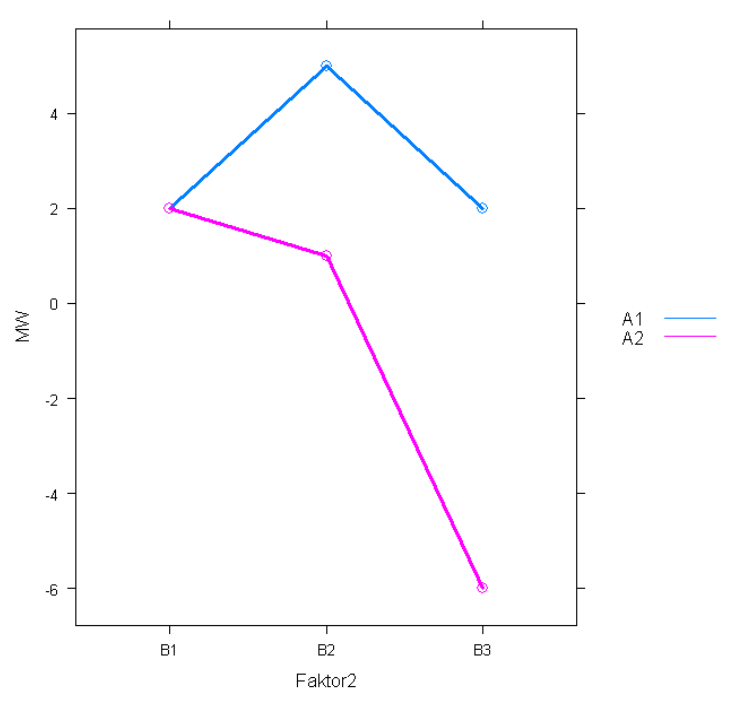
\includegraphics[width=0.8\linewidth]{fig/Interaktion_Plot.png} 
        \end{center}

        \vspace{2mm}

        In beiden Fällen werden folgende Gleichungen erfüllt:
        \begin{align*}
        &\wh{\mu} + \wh{\tau_1} + \wh{\gamma_1} + \wh{( \tau \gamma )}_{1,1} = 2\\
        &\wh{\mu} + \wh{\tau_1} + \wh{\gamma_2} + \wh{( \tau \gamma )}_{1,2} = 5\\
        &\wh{\mu} + \wh{\tau_1} + \wh{\gamma_3} + \wh{( \tau \gamma )}_{1,3} = 2\\
        &\wh{\mu} + \wh{\tau_2} + \wh{\gamma_1} + \wh{( \tau \gamma )}_{2,1} = 2\\
        &\wh{\mu} + \wh{\tau_2} + \wh{\gamma_2} + \wh{( \tau \gamma )}_{2,2} = 1\\
        &\wh{\mu} + \wh{\tau_2} + \wh{\gamma_3} + \wh{( \tau \gamma )}_{2,3} = -6
        \end{align*}

        \textbf{Effekt-Kodierung:}
        \begin{align*}
        \wh{\mu} &= 1 & \wh{\gamma_1} &= 1 & \wh{( \tau \gamma )}_{1,1} &= -2 & \wh{( \tau \gamma )}_{2,1} &= 2\\
        \wh{\tau_1} &= 2 & \wh{\gamma_2} &= 2 & \wh{( \tau \gamma )}_{1,2} &= 0 & \wh{( \tau \gamma )}_{2,2} &= 0\\
        \wh{\tau_2} &= -2 & \wh{\gamma_3} &= -3 & \wh{( \tau \gamma )}_{1,3} &= 2 & \wh{( \tau \gamma )}_{2,3} &= -2
        \end{align*}
        
        \vspace{2mm}

        \textbf{Referenz-Kodierung:}
        \begin{align*}
        & \wh{\mu} = -6  & \wh{\gamma_1} &= 8 & \wh{( \tau \gamma )}_{1,1} &= -2 & \wh{( \tau \gamma )}_{2,1} &= 0\\
        & \wh{\tau_1} = 8 & \wh{\gamma_2} &= 7 & \wh{( \tau \gamma )}_{1,2} &= 1 & \wh{( \tau \gamma )}_{2,2} &= 0\\
        & \wh{\tau_2} = 0 & \wh{\gamma_3} &= 0 & \wh{( \tau \gamma )}_{1,3} &= 0 & \wh{( \tau \gamma )}_{2,3} &= 0
        \end{align*}

        \end{minipage}
    };
%------------ Visualisierung Beispiel Header ---------------------
\node[fill = blue, text=white, font=\bfseries, right=10pt] at (box.north west) 
{Visualisierung Beispiel};
\end{tikzpicture}

%------------ Kodierung Vergleich (mehrfaktoriell) Beispiel---------------
\begin{tikzpicture}
    \node [mybox] (box){%
        \begin{minipage}{0.3\textwidth}
        Sei $K_C = 2$ und $K_D = 3$ mit $n_{k,l} = 2$ für alle $k=1,2,3$ und $l=1,2$.\\
        Dann erhalten wir als Designmatrix für das Modell mit Interaktionstermen\\
        \vspace{2mm}

        \textbf{Effekt-Kodierung}:
        $$\begin{pmatrix} \bX^e & \bZ^e \end{pmatrix} = \begin{pmatrix}
            1 & 1 & 1 & 0 & 1 & 0\\ 
            1 & 1 & 1 & 0 & 1 & 0\\
            1 & 1 & 0 & 1 & 0 & 1\\
            1 & 1 & 0 & 1 & 0 & 1\\
            1 & 1 & -1 & -1 & -1 & -1\\ 
            1 & 1 & -1 & -1 & -1 & -1\\
            1 & -1 & 1 & 0 & -1 & 0\\
            1 & -1 & 1 & 0 & -1 & 0\\
            1 & -1 & 0 & 1 & 0 & -1\\
            1 & -1 & 0 & 1 & 0 & -1\\
            1 & -1 & -1 & -1 & 1 & 1\\
            1 & -1 & -1 & -1 & 1 & 1
        \end{pmatrix}$$

        \vspace{2mm}
        \textbf{Referenz-Kodierung}:
        $$\begin{pmatrix} \bX & \bZ \end{pmatrix} = \begin{pmatrix}
            1 & 1 & 1 & 0 & 1 & 0\\
            1 & 1 & 1 & 0 & 1 & 0\\
            1 & 1 & 0 & 1 & 0 & 1\\
            1 & 1 & 0 & 1 & 0 & 1\\
            1 & 1 & 0 & 0 & 0 & 0\\
            1 & 1 & 0 & 0 & 0 & 0\\
            1 & 0 & 1 & 0 & 0 & 0\\
            1 & 0 & 1 & 0 & 0 & 0\\
            1 & 0 & 0 & 1 & 0 & 0\\
            1 & 0 & 0 & 1 & 0 & 0\\ 
            1 & 0 & 0 & 0 & 0 & 0\\
            1 & 0 & 0 & 0 & 0 & 0
        \end{pmatrix}$$
        \end{minipage}
    };
%------------ Modell mit Kodierung Vergleich (mehrfaktoriell) Beispiel Header ---------------------
\node[fill = blue, text=white, font=\bfseries, right=10pt] at (box.north west) 
{Kodierung Vergleich (mehrfaktoriell) Beispiel};
\end{tikzpicture}

%------------ Interaktionsmodell mit stetigen Merkmalen (Kovarianzanalyse) Interpretation ---------------
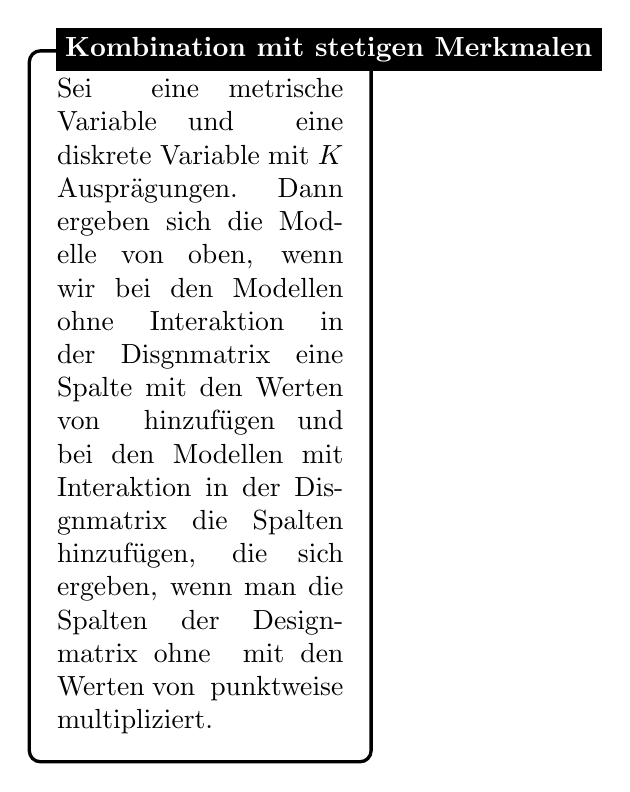
\begin{tikzpicture}
    \node [mybox] (box){%
        \begin{minipage}{0.3\textwidth}
        Sei $\bE$ eine metrische Variable und $\bC$ eine diskrete Variable mit $K$ Ausprägungen.
        Dann ergeben sich die Modelle von oben, wenn wir bei den Modellen ohne Interaktion in der Disgnmatrix eine Spalte 
        mit den Werten von $\bE$ hinzufügen und bei den Modellen mit Interaktion in der Disgnmatrix die Spalten hinzufügen, 
        die sich ergeben, wenn man die Spalten der Designmatrix ohne $\bE$ mit den Werten von $\bE$ punktweise multipliziert.

        \end{minipage}
    };
%------------ Interaktionsmodell stetigen Merkmalen (Kovarianzanalyse) Header ---------------------
\node[fill = black, text=white, font=\bfseries, right=10pt] at (box.north west) 
{Kombination mit stetigen Merkmalen};
\end{tikzpicture}


\end{multicols*}